\section*{Porównanie wyników eksperymentów symulacyjnych oraz z wykorzystaniem rzeczywistych robotów}
\begin{frame}
\frametitle{\secname}
\framesubtitle{Otwarta przestrzeń ustawienie prostopadłe}
\begin{figure}[ht] % h:here; t:top; b:bottom; p:page; default:ht
	\captionsetup[subfigure]{labelformat=empty}
	\centering
	\subfloat[][Symulacja 1-2]
{
	\includegraphics[page = 2, width=0.49\textwidth]{img/Simulation_Open_space.pdf}
}
	\subfloat[][Roboty 1-2]
{
	\includegraphics[page = 2, width=0.49\textwidth]{img/Robots_Open_space.pdf}
}
\end{figure}


\note{

\begin{itemize}
	\item Wiele czynników mają wpływ na różnice pomiędzy czasami uzyskanymi w symulacji a na rzeczywistych robotach. Możemy do nich zaliczyć między innymi:
	
	\item W symulatorze ruch robotów jest ,,idealny''. Nawet obrót o niewielki kąt zmienia jego pozycje. Na rzeczywistych robotach nie jesteśmy tego tak precyzyjnie uzyskać, choćby ze względu na poślizgi robotów.
	
	\item Opóźnienie na sieci związane z odbieraniem wysłaniem wiadomości.  Brak ich w symulacji gdyż jest to pojedynczy komputer.
	\item Różne czasy wykonywania obliczeń (niezależne maszyny) i podejmowanych decyzji które muszą być wielokrotnie zmieniane gdyż roboty przemieściły się i trzeba to uwglednić.
	
	\item Niedokładność wynikająca z lokalizacji - pozycja robotów lekko ,,pływają'' co nie występuje w symulacji tu pozycja jest zawsze pewna.
	
	\item Jeśli chodzi o czas wykonania to związany jest z innymi prędkościami robotów w symulacji a na rzeczywistych robotach. 
	\item Wielkość laboratorium nie była odwzorowywana w symulatorze.
\end{itemize}

}

\end{frame}


\section*{Porównanie wyników eksperymentów symulacyjnych oraz z wykorzystaniem rzeczywistych robotów}
\begin{frame}
\frametitle{\secname}
\framesubtitle{Przejście przez drzwi}
\begin{figure}[ht] % h:here; t:top; b:bottom; p:page; default:ht
	\captionsetup[subfigure]{labelformat=empty}
	\centering
		\subfloat[][Symulacja 1-H2]
{
	\includegraphics[page = 2, width=0.49\textwidth]{img/Simulation_Passage_through_the_door.pdf}
}
	\subfloat[][Roboty 1-H2]
{
	\includegraphics[page = 2, width=0.49\textwidth]{img/Robots_Passage_through_the_door.pdf}
}
\end{figure}
\end{frame}
